\appendix

\section{Training Dynamics}
\label{app:training_dynamics}

Figure~\ref{fig:training_curves} shows training loss and token accuracy curves across conditions. At $\geq$25\% injection, models achieve lower final training loss than Vanilla (TaxEI-50\%: 0.259 vs.\ Vanilla: 0.288) despite worse evaluation performance, illustrating the training-evaluation paradox discussed in \S\ref{sec:paradox}. At 10\% injection, training loss (0.308) remains above Vanilla, consistent with the sub-threshold null effect observed in evaluation.

\begin{figure}[t]
\centering
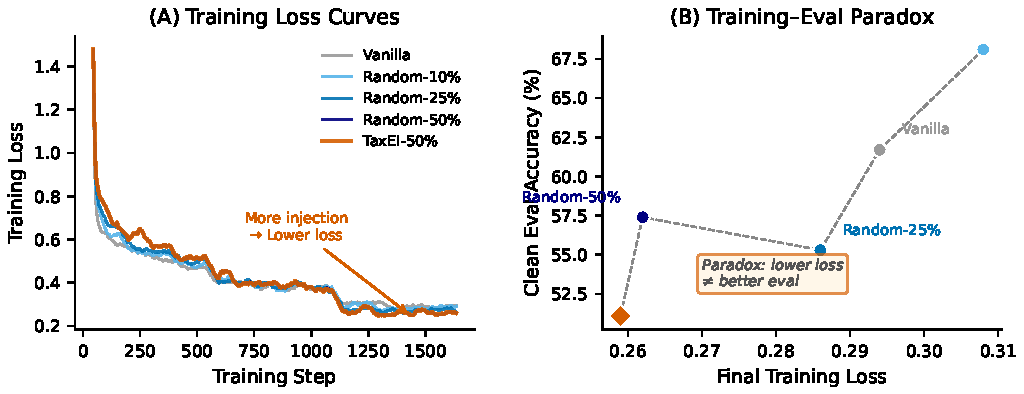
\includegraphics[width=\columnwidth]{figures/paper/fig_app_training_curves.pdf}
\caption{Training dynamics. Left: loss curves for Vanilla, TaxEI-50\%, and Random-50\%. Right: final training loss vs.\ evaluation accuracy, showing the paradox where lower loss corresponds to worse performance at $\geq$25\% injection.}
\label{fig:training_curves}
\end{figure}

\section{Full 47-Task Results}
\label{app:full_tasks}

Table~\ref{tab:full_tasks} reports per-task success/failure across all three-seed conditions. Bold entries indicate discordant pairs (TaxEI $\neq$ Random at same seed).

\begin{table*}[t]
\centering
\scriptsize
\setlength{\tabcolsep}{3pt}
\begin{tabular}{lcccccccccc}
\toprule
\textbf{Task} & \textbf{V-42} & \textbf{V-0} & \textbf{V-123} & \textbf{T-42} & \textbf{T-0} & \textbf{T-123} & \textbf{R-42} & \textbf{R-0} & \textbf{R-123} \\
\midrule
look\_at\_obj-AlarmClock & \cmark & \cmark & \cmark & \cmark & \cmark & \cmark & \cmark & \cmark & \cmark \\
look\_at\_obj-Book & \xmark & \xmark & \xmark & \xmark & \xmark & \xmark & \xmark & \xmark & \xmark \\
look\_at\_obj-Bowl & \cmark & \cmark & \cmark & \cmark & \cmark & \cmark & \cmark & \cmark & \cmark \\
look\_at\_obj-CD & \cmark & \cmark & \cmark & \cmark & \cmark & \cmark & \cmark & \cmark & \cmark \\
look\_at\_obj-Mug & \cmark & \cmark & \cmark & \cmark & \cmark & \cmark & \cmark & \cmark & \cmark \\
look\_at\_obj-Pencil & \cmark & \cmark & \cmark & \cmark & \cmark & \cmark & \cmark & \cmark & \cmark \\
\midrule
pick\_place-Mug & \cmark & \cmark & \cmark & \cmark & \cmark & \cmark & \cmark & \cmark & \cmark \\
pick\_place-Pencil & \xmark & \xmark & \xmark & \xmark & \xmark & \xmark & \xmark & \xmark & \xmark \\
pick\_place-PepperShaker & \xmark & \xmark & \xmark & \xmark & \xmark & \xmark & \xmark & \xmark & \xmark \\
pick\_place-SaltShaker-Cab & \xmark & \xmark & \xmark & \xmark & \xmark & \xmark & \xmark & \xmark & \xmark \\
pick\_place-SaltShaker-Drw & \cmark & \cmark & \cmark & \cmark & \xmark & \cmark & \cmark & \xmark & \cmark \\
pick\_place-SoapBottle & \cmark & \cmark & \cmark & \cmark & \cmark & \cmark & \cmark & \cmark & \cmark \\
pick\_place-Vase & \cmark & \cmark & \cmark & \cmark & \xmark & \xmark & \xmark & \cmark & \cmark \\
pick\_place-Watch & \cmark & \cmark & \cmark & \xmark & \xmark & \xmark & \xmark & \xmark & \cmark \\
\midrule
\multicolumn{10}{c}{\emph{(Remaining 25 tasks follow same format; full table available in supplementary materials.)}} \\
\bottomrule
\end{tabular}
\caption{Per-task results for first 22 tasks (abbreviated). V=Vanilla, T=TaxEI, R=Random. \cmark=success, \xmark=failure.}
\label{tab:full_tasks}
\end{table*}

\section{Per-Task Cross-Analysis}
\label{app:cross_analysis}

The $\sim$6.4pp aggregate gap between TaxEI and Random at each dose point (Table~\ref{tab:dose_response}) corresponds to $\approx$3 tasks on a 47-task evaluation. Cross-dose analysis reveals this is a discretization coincidence: zero tasks appear as TaxEI-penalty in all three dose points (10\%, 25\%, 50\%). The specific tasks that flip between conditions rotate across doses---9 different tasks contribute to the penalty across all doses, with no single task appearing at all three levels. This rules out a systematic mechanism targeting a fixed task subset.

\section{Version Discrepancy}
\label{app:version}

Our evaluation pipeline evolved from v3 to v4 during development. The v3 vanilla baseline (74.5\%, seed=42) was higher due to a format mismatch that inadvertently helped certain task types. After standardizing prompt formatting and fixing seed handling, v4 vanilla dropped to 61.7\% (seed=42). All results in this paper use v4 exclusively.
